En este trabajo nos hemos centrado principalmente en la aplicación de algoritmos de clasificación de aprendizaje supervisado para las etiquetas relacionadas con las disfunciones cognitivas presentes en los datos proporcionados. Los experimentos que se ha llevado persiguen el objetivo de obtener el mejor modelo para cada algoritmos a partir de un conjunto de datos usados para su entrenamiento.

\section{Obtención de los modelos}

Los modelos de aprendizaje automático se generan a través de la implementación de un algoritmo junto a sus parámetros que lo configuran aplicado a un subconjunto de atributos. Por lo tanto, hay que elegir el algoritmo, sus parámetros y los atributos de los datos para poder describir cada modelo. A su vez, un modelo puede estar compuesto de varios pasos configurables que transforman los datos organizados en fases consecutivas.

\section{Algoritmos}

Dentro de la amplia familia de los algoritmos de clasificación de aprendizaje supervisado nos encontramos multitud de algoritmos con sus variantes donde ninguno es, a priori, más adecuado que otro: ``no free lunch theorem'' \cite{Wolpert1996TheAlgorithms}. Centrándonos en las implementaciones proporcionadas por los frameworks de aprendizaje automático scikit-learn \cite{Scikit-learn:Documentation} y Keras \cite{KerasDocumentation}, se han realizado una valoración inicial de los algoritmos seleccionando finalmente ``Logistic Regression'', ``Support Vector Machine'', ``Gaussian Naive Bayes'', ``Random Forest Classifier'' y ``Artificial Neural Network''.

\subsection{Logistic Regression}
Usado extensamente en las ciencias médicas y sociales, este algoritmo se basa en una clasificación  lineal donde las probabilidades que describen los posibles resultados de un único ensayo se modelan utilizando una función logística. En la imagen \ref{alglog} se puede ver un ejemplo gráfico de su aplicación.

\begin{figure}[H]
\centering
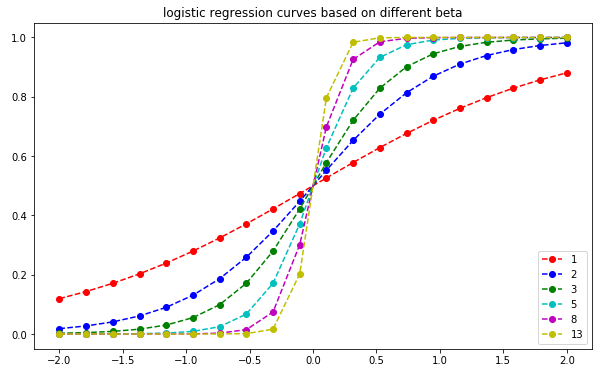
\includegraphics[width=0.74\textwidth]{figs/algorimos/log.png}
\caption{Algoritmo Logistic Regression \cite{MachineHEURISTICS}}
\label{figure:alglog}
\end{figure}

\subsection{Support Vector Machine}

Como se puede consultar en \cite{Brown2016MachineMRI} \gls{svm} es un algoritmo de aprendizaje supervisado muy utilizado para investigaciones relacionadas con la neuroimagen. Tiene la característica de ser muy eficiente cuando el número de atributos es alto ya que está basado en la minimización del riesgo estructural. Este algoritmo representa las instancias de la muestra como puntos en el espacio el cual es dividido por un hiperplano. En base a esta división se establecen las etiquetas a los valores (figura \ref{figure:algsvm}).

\begin{figure}[H]
\centering
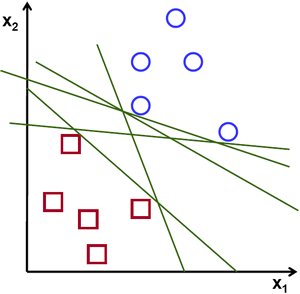
\includegraphics[width=0.3\textwidth]{figs/algorimos/svm.png}
\caption{Ejemplo algoritmo \gls{svm} \cite{IntroductionDocumentation}}
\label{figure:algsvm}
\end{figure}

\subsection{Gaussian Naive Bayes}

Este modelo es clasificador probabilístico fundamentado en el teorema de Bayes,  supone que la presencia o ausencia de una característica particular no está relacionada con la presencia o ausencia de cualquier otra característica, dada la clase variable \cite{de:NaiveClassifier}. 

\subsection{Random Forest Classifier}
Modelo compuesto por la combinación de árboles predictores tal que cada árbol depende de los valores de un vector aleatorio probado independientemente y con la misma distribución para cada uno de estos \cite{Breiman2001RandomForests}. 

\subsection{Artificial Neural Network}
Este modelo se caracteriza por su organización en capas de neuronas donde cada una
propaga los resultados a la siguiente en función a unas reglas configuradas. Dependiendo del la configuración de estas reglas y capas define la complejidad del modelo. En la imagen \ref{figure:ann} podemos ver un ejemplo con tres capas.

\begin{figure}[H]
\centering
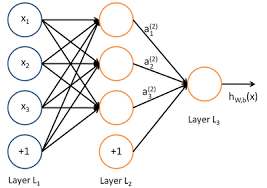
\includegraphics[width=0.5\textwidth]{figs/algorimos/ann.png}
\caption{Ejemplo \gls{ann} con tres capas}
\label{figure:ann}
\end{figure}

\section{Reducción de la dimensionalidad}

En este trabajo nos encontramos con unos datos con muy alta dimensionalidad. Sin contar otros atributos disponibles en la hoja de cálculo, disponemos de 6 matrices con 76x76 celdas cada una, es decir, más de 35.000 atributos por cada ejemplar. Para reducir esta dimensionalidad se han seguido los siguientes pasos durante los experimentos:

\begin{enumerate}
    \item Selección conjunto de matrices para ser usadas como datos para los modelos a través de combinaciones, esto implica el descarte de matrices en su conjunto con todos sus valores.
    
    \item Combinación de los valores de las matrices en una única Por ejemplo, usar todas las matrices disponibles para las instancias para la creación de una única matriz con los valores de la media ponderada de las 6. Esta matriz sería la usada en el modelo.
    
    \item Reducción de la dimensionalidad a través del algoritmo \gls{pca}.
    
\end{enumerate}

\section{Selección de los parámetros y atributos}

Cada algoritmo tiene su propio conjunto de parámetros que lo configuran. A su vez, a cada uno se le pueden aplicar un conjunto de atributos pudiéndose obtener resultados muy diversos. Igualmente, cada paso en el preprocesado de los datos explicado con anterioridad tiene sus propios parámetros. Todo esto hace que la elección del modelo óptimo para un algoritmo establecido no es un problema trivial.

Dado el número de combinaciones posibles entre los parámetros de cada modelo, la búsqueda exhaustiva de todos ellos tiene un coste inasumible para este trabajo. A través de la elección de estos aleatoriamente usando la utilidad de scikit-learn ``Randomized Parameter Optimization'' obtenemos una aproximación al modelo óptimo y a la configuración de los pasos previos.

\section{Validación de los modelos}
Tanto para comparar los posibles modelos obtenidos durante la selección de parámetros y atributos y para validar el modelo seleccionado para compararlo con otros se usa la implementación en scikit-learn de la técnica validación \gls{kfold} estratificada (Stratified \gls{kfold}). La estratificación es muy importante para los algoritmos de clasificación con muestras con pocos ejemplares para conservar el porcentaje de elementos de cada clase en los conjuntos.

Esta técnica de validación descompone el conjunto inicial en dos, entrenamiento y test. El primero es usado para seleccionar el modelo. El conjunto de test para validar el modelo seleccionado, medir su exactitud y comprobar que no se produce sobreajuste (overfitting).

Durante la selección de los parámetros, el algoritmo ``Randomized Parameter Optimization'' realiza igualmente \gls{kfold}  estratificada sobre el conjunto de entrenamiento para comparar los candidatos entre ellos. Es decir, vuelve a dividir en cada combinación de parámetros establecida el conjunto de entrenamiento previamente obtenido. Como resultado se obtiene un conjunto de entrenamiento para el modelo y otro de test, que en este caso se suele llamar conjunto de validación. Este conjunto es usado para comprobar la adecuación de la combinación de atributos que se está probando (ver imagen \ref{figure:kfold}).

\begin{figure}[H]
\centering
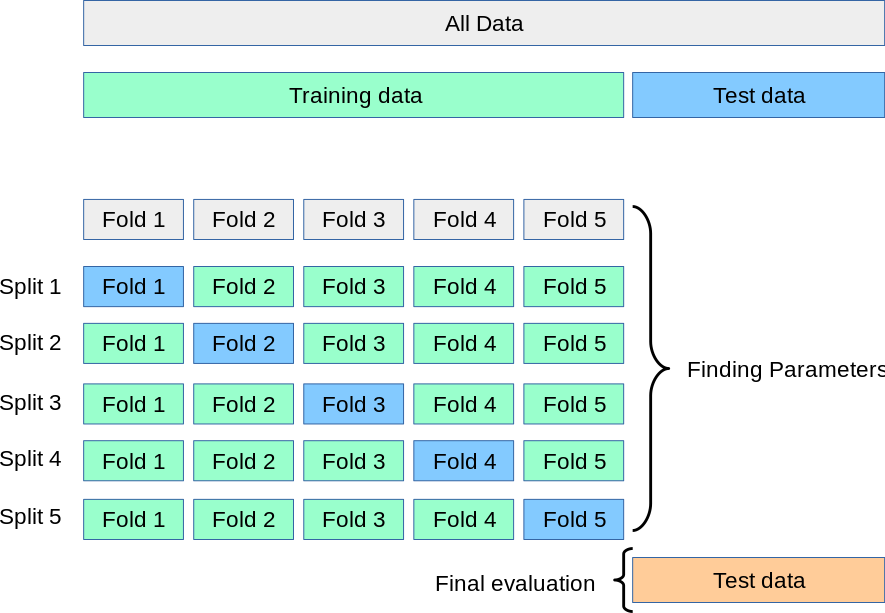
\includegraphics[width=0.74\textwidth]{figs/experimentos/kfold.png}
\caption{Ejemplo \gls{kfold} para seleccionar el modelo y la evaluación final \cite{GitHubCompleto}}
\label{figure:kfold}
\end{figure}
